\documentclass[pdf,notheorems,10pt,intlimits,unicode]{beamer}
\usetheme[numbers,totalnumbers,compress,nologo]{Statmod}
\usefonttheme[onlymath]{serif}
\setbeamertemplate{navigation symbols}{}

\usepackage[utf8]{inputenc}
\usepackage[T2A]{fontenc}
\usepackage[russian]{babel}

\usepackage{graphicx,subcaption,ragged2e}
\usepackage{caption}
\usepackage{slashbox}

\usepackage{tikz}
\usepackage{hhline}
\usepackage{array}
\usepackage[table,x11names]{xcolor}

\usepackage{amsthm}
\usepackage{amsmath}
\usepackage{amssymb}
\usepackage{mathtools}
\usepackage{hhline}
\usepackage{xcolor}
\usepackage{array}
\usepackage{bbm}
\usepackage{bm}

\AtBeginSection[]{
  \begin{frame}[noframenumbering]
  \vfill
  \centering
  \begin{beamercolorbox}[sep=8pt,center,shadow=true,rounded=true]{title}
    \usebeamerfont{title}\insertsectionhead\par%
  \end{beamercolorbox}
  \vfill
  \end{frame}
}

\setbeamerfont{institute}{size=\normalsize}
\setbeamercolor{bluetext_color}{fg=blue}

\newtheorem{remark}{Замечание}
\newtheorem{algorithm}{Алгоритм}
\newtheorem{assumption}{Предположение}
\newtheorem{definition}{Определение}

\newcommand{\bfxi}{\boldsymbol{\xi}}
\newcommand{\bluetext}[1]{{\usebeamercolor[fg]{bluetext_color}#1}}
\newcommand{\redtext}[1]{{\usebeamercolor[fg]{redtext_color}#1}}

\setcounter{tocdepth}{2}

\title{Автоматическое разложение временного ряда на тренд, периодичности и шум, используя метод Monte Carlo SSA}

\author{Потешкин Е.П., Голяндина Н.Э.}

\institute[Санкт-Петербургский Государственный Университет]{%
	\small
	Санкт-Петербургский государственный университет\\
	Кафедра статистического моделирования
}

\date{\\Список-2026\\30 апреля 2026, Санкт-Петербург}

\input{letters_series_mathbb.tex}

\begin{document}

\begin{frame}[plain]
    \titlepage
    \note{Научный руководитель  д.ф.-м.н., доцент Голяндина\,Н.\,Э.,\\
        кафедра статистического моделирования}
\end{frame}

\begin{frame}{Введение}

    $\tX=(x_1,\ldots,x_N)$~--- временной ряд длины $N$.\medskip

    \bluetext{Модель}: $\tX=\tT+\tP+\tR$, где $\tT$~--- тренд, $\tP$~--- периодическая компонента и $\tR$~--- шум, случайная составляющая.\medskip

    \bluetext{Проблема}: Как выделить сигнал $\tS=\tT+\tP$?\medskip

    \bluetext{Метод}: Singular spectrum analysis (SSA)~[Broomhead and King, 1986; Golyandina, Nekrutkin and Zhigljavsky, 2001].\medskip

    \bluetext{Преимущества}:
    \begin{enumerate}
        \item Не требует задания модели сигнала и шума, в частности, периодов цикличности.
        \item Позволяет строить прогноз и заполнять пропуски.
    \end{enumerate}\smallskip

    \textcolor{red}{Проблема}: один из шагов SSA требует визуального анализа для определения сигнальных компонент, необходима автоматизация этого шага.

\end{frame}

\begin{frame}{Обозначения и известные результаты: Метод SSA}

    \bluetext{Входные данные}: временной ряд $\tX=(x_1,\ldots,x_N)$.\medskip

    \bluetext{Параметры}: длина окна $L$, $1<L<N$, набор индексов $I\subset\{1,\ldots, d\}$.\medskip

    \bluetext{Результат}: оценка сигнала $\hat\tS$.\medskip
    \begin{enumerate}
        \item \textbf{Вложение}: $\bfX=\cT(\tX)=[X_1:\ldots:X_K]$, где $X_i=(x_1,\ldots,x_{i+L-1})^\rmT$, $K=N-L+1$.\smallskip
        \item \textbf{Разложение}: $\bfX=\sum_{i=1}^r \sigma_i U_i V_i^\rmT=\bfX_1+\ldots+\bfX_r$, $\operatorname{rank}\bfX_i=1$, $(\sigma_i, U_i, V_i)$~--- $i$-ая сингулярная тройка.\smallskip
        \item \textbf{Группировка}: $\bfX=\bfX_{I}+(\bfX - \bfX_{I})$, где $\bfX_{I}=\sum_{i\in I}\bfX_i$.\smallskip
        \item \textbf{Восстановление}: $\tX=\hat{\tS}+\hat{\tR}$, где $\hat\tS=\cT^{-1}\circ\cH(\bfX_{I})$.
    \end{enumerate}

\end{frame}

\begin{frame}{Обозначения и известные результаты: Метод SSA-Aid~[Golyandina, Dudnik and Shlemov, 2023; Дудник, 2025]}

    \begin{figure}
        \centering
        
\includegraphics[width=0.82\textwidth]{img/ssa_aid_flowchart.pdf}
        \caption{Блок-схема метода SSA-Aid}
    \end{figure}
    
\end{frame}

\begin{frame}{Идеи, заложенные в SSA-Aid}

    \begin{itemize}
        \item Поскольку тренду соответствуют низкие частоты, \textbf{PAI$\mathbf{\left( [0, \bm\omega_0), T_0\right)}$} отбирает те компоненты, доля значений периодограммы которых в частотах из $[0, \omega_0)$ больше некоторого порога $T_0$.
        \item Поскольку трендовые компоненты могут смешаться с периодическими, перед выделением тренда применяется алгоритм улучшения разделимости \textbf{EOSSA}~[Шлемов, 2017; Golyandina, Dudnik and Shlemov, 2023].
        \item Для идентификации периодических компонент используется \textbf{метод регулярности углов}~[Жорникова, 2018; Дудник, 2025]: метод использует факт, что углы между последовательными отрезками на двумерной диаграмме сингулярных векторов равны.
        \item Поскольку EOSSA делает шумовые компоненты похожими на периодики, для отбора периодик дополнительно используется \textbf{статистический критерий} проверки гипотезы об отсутствии сигнала в остатке.
    \end{itemize}

\end{frame}

\begin{frame}{SSA-Aid: пример}
    \begin{figure}
        \centering
        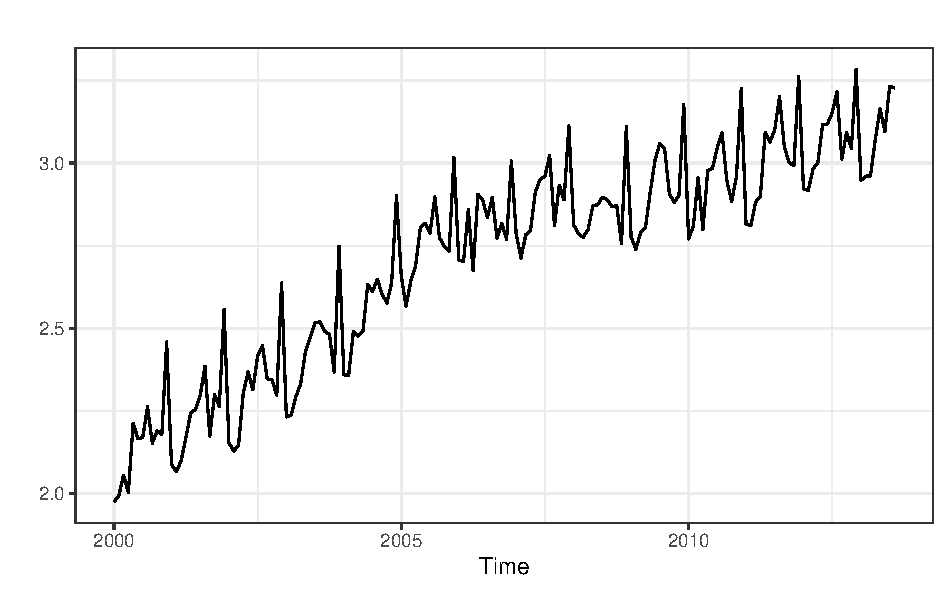
\includegraphics[width=\textwidth]{img/debitcards_plot.pdf}
        \caption{Использование дебетовых карт в розничной торговле в Исландии}
    \end{figure}
\end{frame}

\begin{frame}{SSA-Aid: пример}
    \begin{figure}
        \centering
        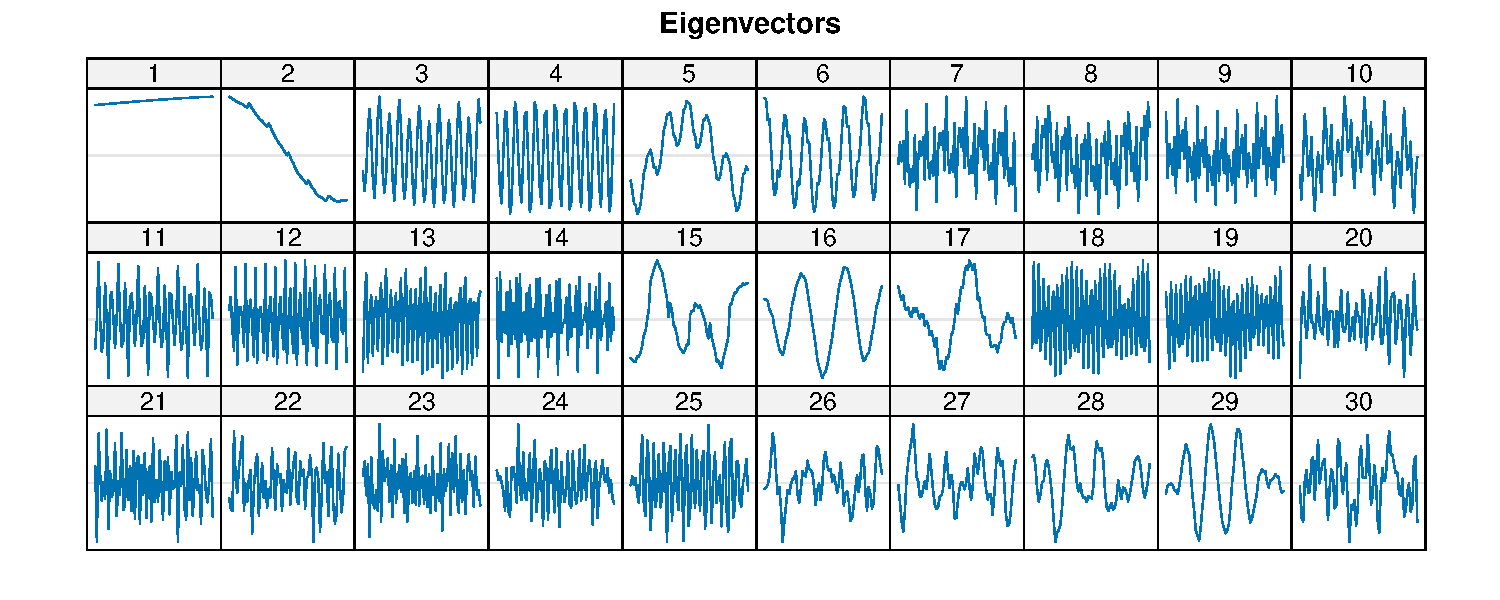
\includegraphics[width=\textwidth]{img/debitcatds_decomposition_basic.pdf}
        \caption{Левые сингулярные векторы $U_i$ до улучшения разделимости}
    \end{figure}

    Компоненты 5--10 смешались с трендом, компоненты сезонности смешались друг с другом.
\end{frame}

\begin{frame}{SSA-Aid: пример}

    \begin{figure}
        \centering
        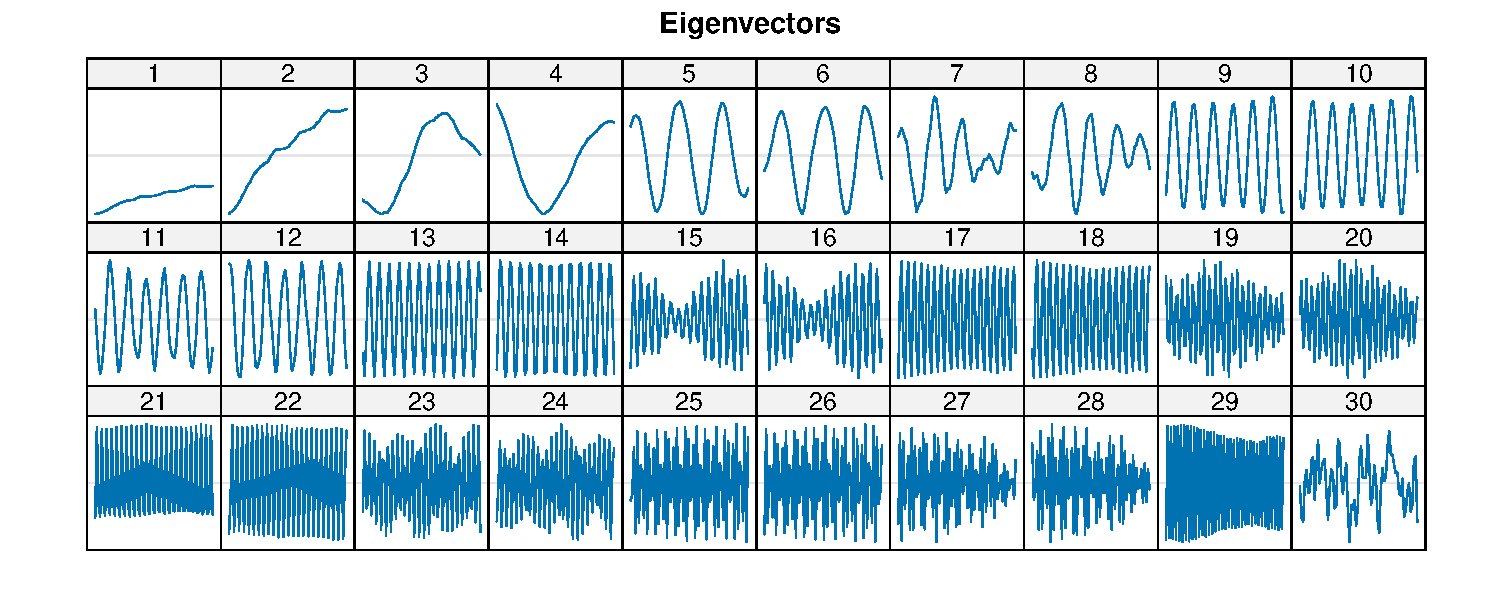
\includegraphics[width=\textwidth]{img/debitcatds_decomposition_eossa.pdf}
        \caption{Левые сингулярные векторы $U_i$ после улучшения разделимости}
    \end{figure}

\end{frame}

\begin{frame}{SSA-Aid: пример}
    \begin{figure}
        \centering
        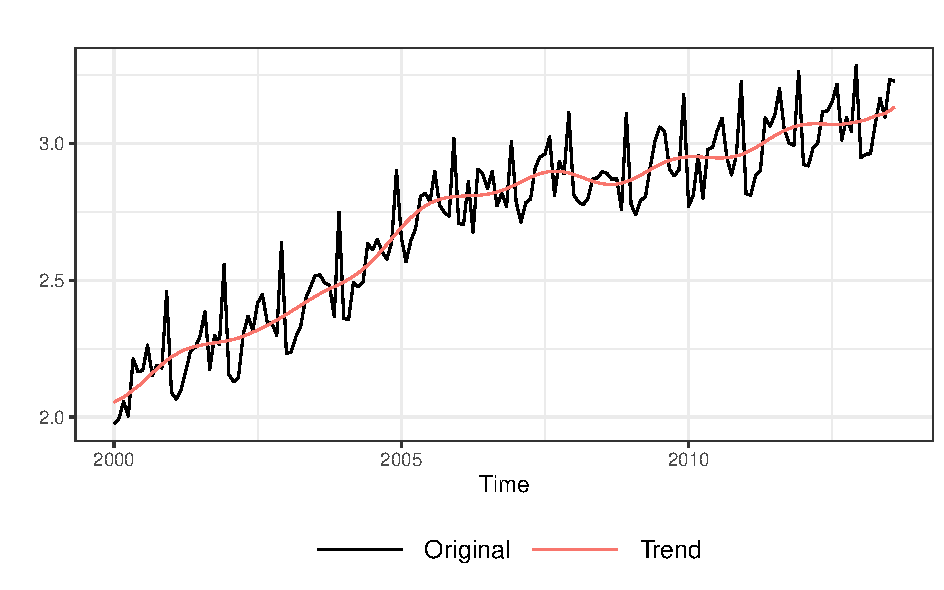
\includegraphics[width=\textwidth]{img/debitcards_auto_trend.pdf}
        \caption{Результат EOSSA($t$) + PAI$\left([0, \omega_0), T_0\right)$ с $t=30$, $\omega_0=1/24$, $T_0=0.5$}
    \end{figure}
\end{frame}

\begin{frame}{SSA-Aid: пример}
    \begin{figure}
        \centering
        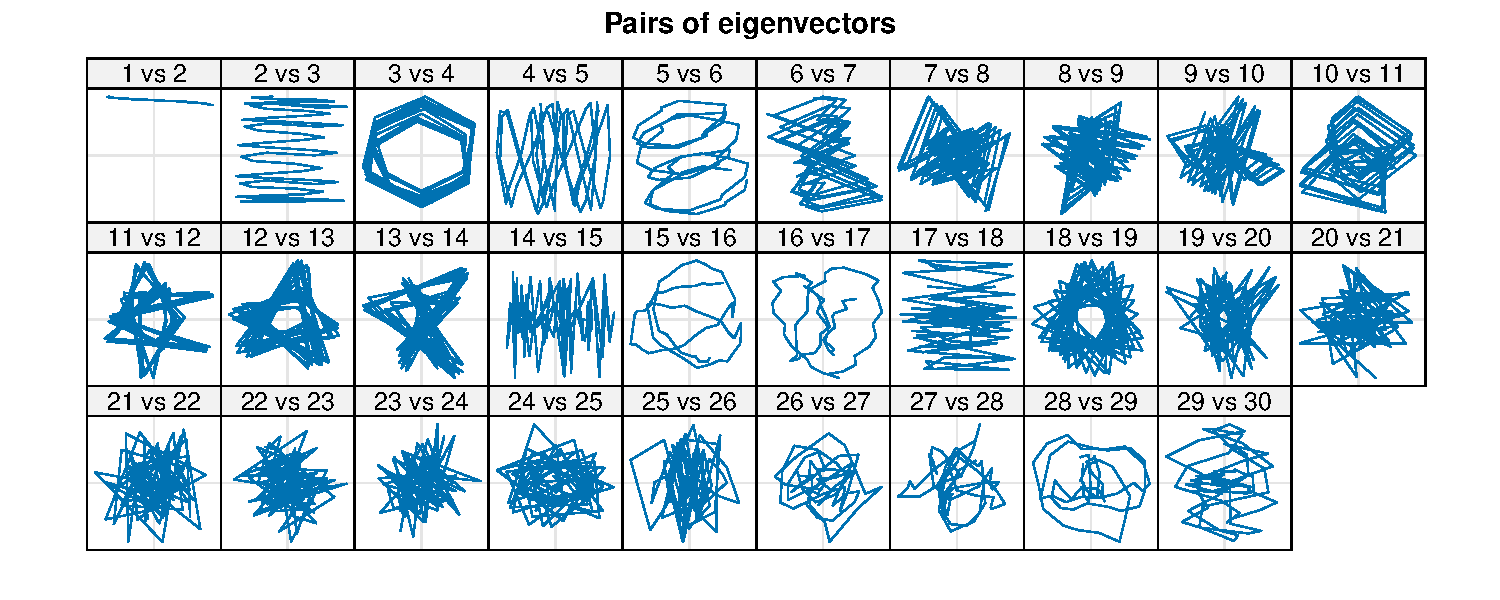
\includegraphics[width=0.95\textwidth]{img/debitcatds_paired_basic.pdf}
        \caption{2D графики левых сингулярных векторов $(U_i, U_{i+1})$ до улучшения разделимости}
    \end{figure}
\end{frame}

\begin{frame}{SSA-Aid: пример}
    \begin{figure}
        \centering
        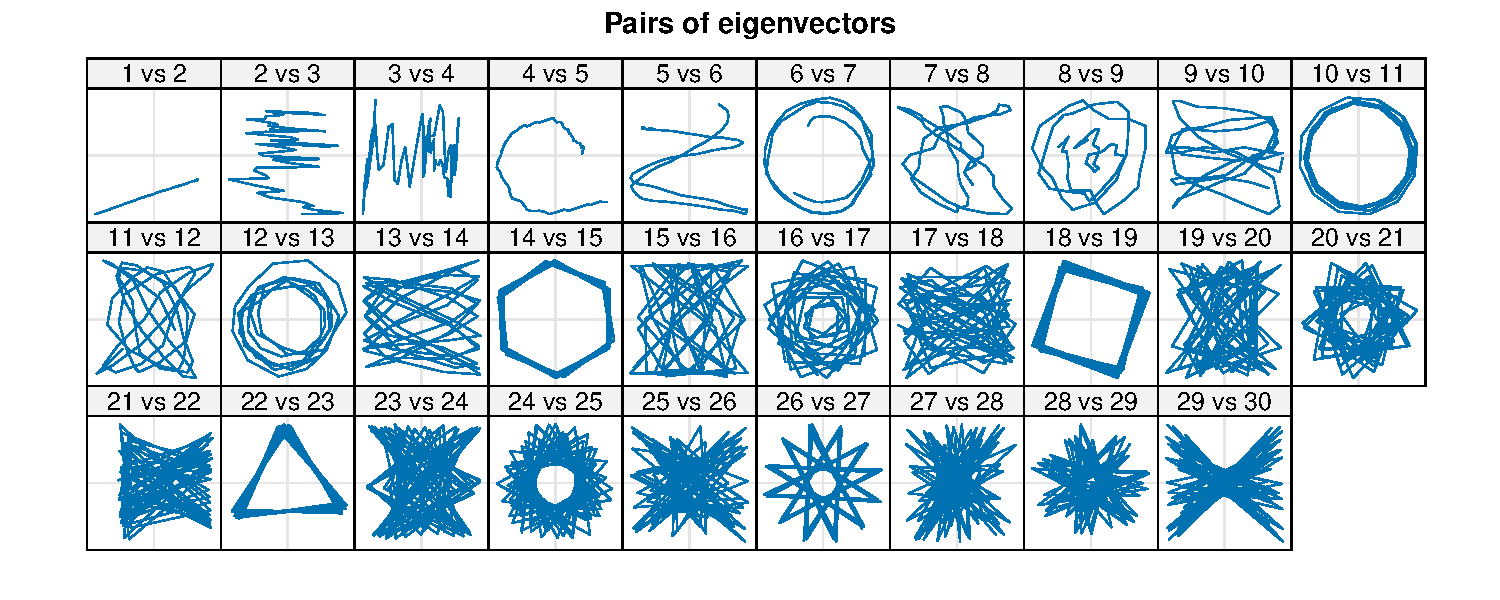
\includegraphics[width=0.92\textwidth]{img/debitcatds_paired_eossa.pdf}
        \caption{2D графики левых сингулярных векторов $(U_i, U_{i+1})$ после улучшения разделимости}
    \end{figure}
    \textcolor{red}{Проблема}: после применения EOSSA некоторые шумовые компоненты стали похожи на периодические.
\end{frame}

\begin{frame}{SSA-Aid: пример}
    \begin{figure}
        \centering
        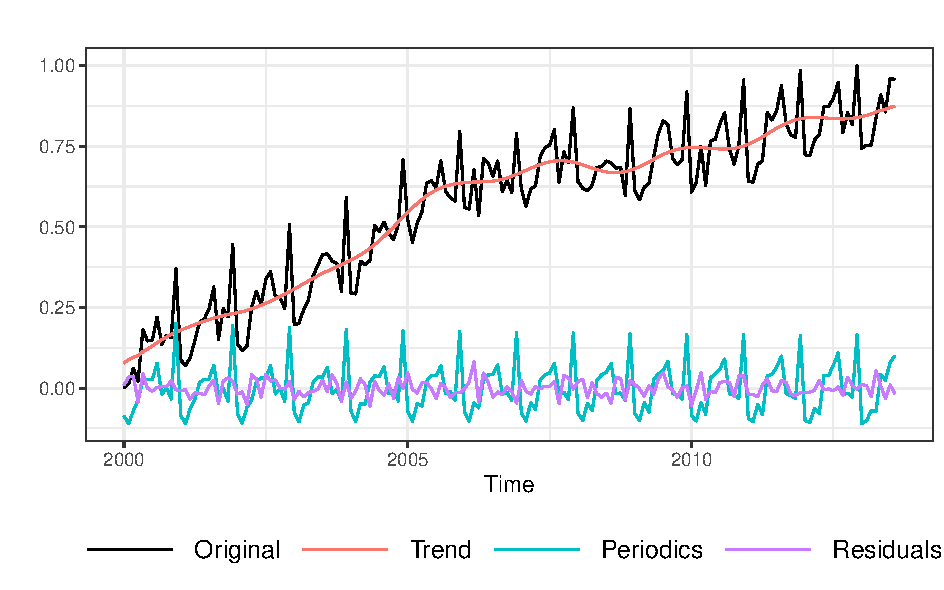
\includegraphics[width=0.92\textwidth]{img/debitcards_ssa_aid.pdf}
        \caption{Результат применения SSA-Aid}
    \end{figure}
\end{frame}

\begin{frame}{Недостатки метода SSA-Aid}

    \bluetext{Допущение}: вклад каждой сигнальной компоненты $>$ вклада любой шумовой $\longrightarrow$ сигналу соответствуют первые компоненты разложения.\medskip
    
    \textcolor{red}{Проблема}: при неравномерном спектре шума (цветной шум) сигнальные компоненты могут оказаться среди шумовых по величине вклада, оставаясь при этом несмешанными с ними.\medskip

    Пусть $\varepsilon_t$~--- белый гауссовский шум, $B$~--- оператор сдвига. Примеры цветного шума:
    \begin{enumerate}
        \item Красный шум:
        \[
        \xi_t=(1-\phi B)^{-1}\varepsilon_t,\quad \phi>0.  
        \]
        \item Процесс с длинной памятью, например, ARFIMA(0, $d$, 0):
        \[
        \xi_t=(1-B)^{-d}\varepsilon_t, \quad d<1/2.
        \]
    \end{enumerate}

\end{frame}

\begin{frame}{Недостатки метода SSA-Aid: пример}

    Модель: $\tX=\tS+\bm\xi$, где $\bm\xi$~--- AR(1) с $\phi=0.7$ и $\sigma^2=1$, $N=200$,
    \[
    s_n=0.075e^{0.02n}\cos(2\pi n / 8) + 1.2\cos(2\pi n / 4) + 0.25\cdot (-1)^n.
    \]

    \begin{figure}
        \centering
        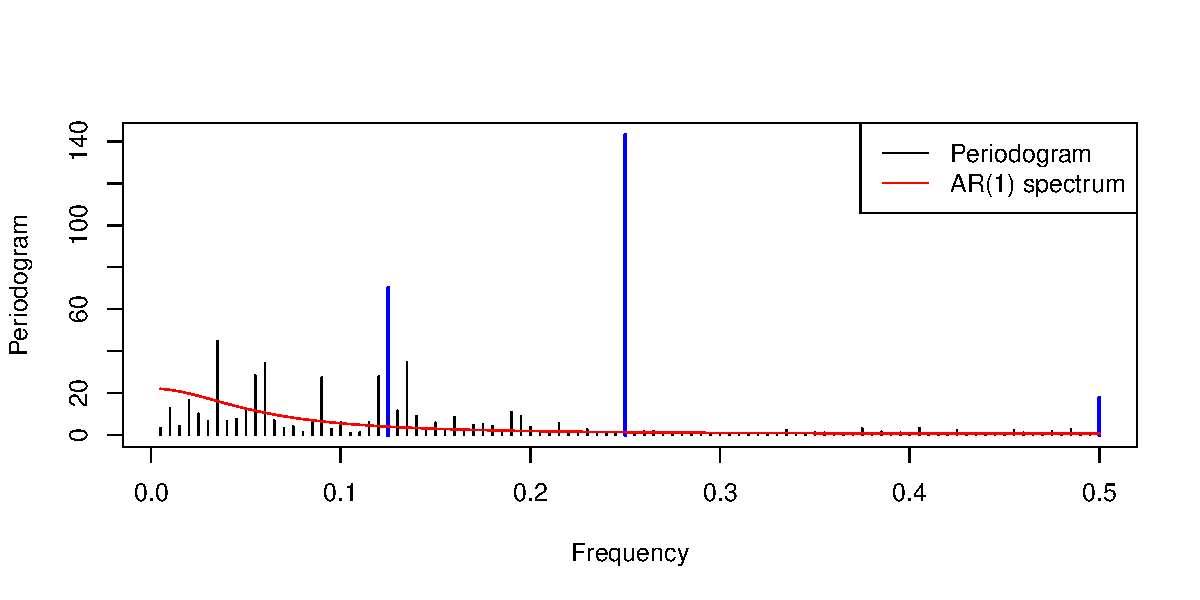
\includegraphics[width=\textwidth]{img/non_dominant_signal_pgram.pdf}
        \caption{Периодограмма ряда}
    \end{figure}

\end{frame}

\begin{frame}{Недостатки метода SSA-Aid: пример}

    \begin{figure}
        \centering
        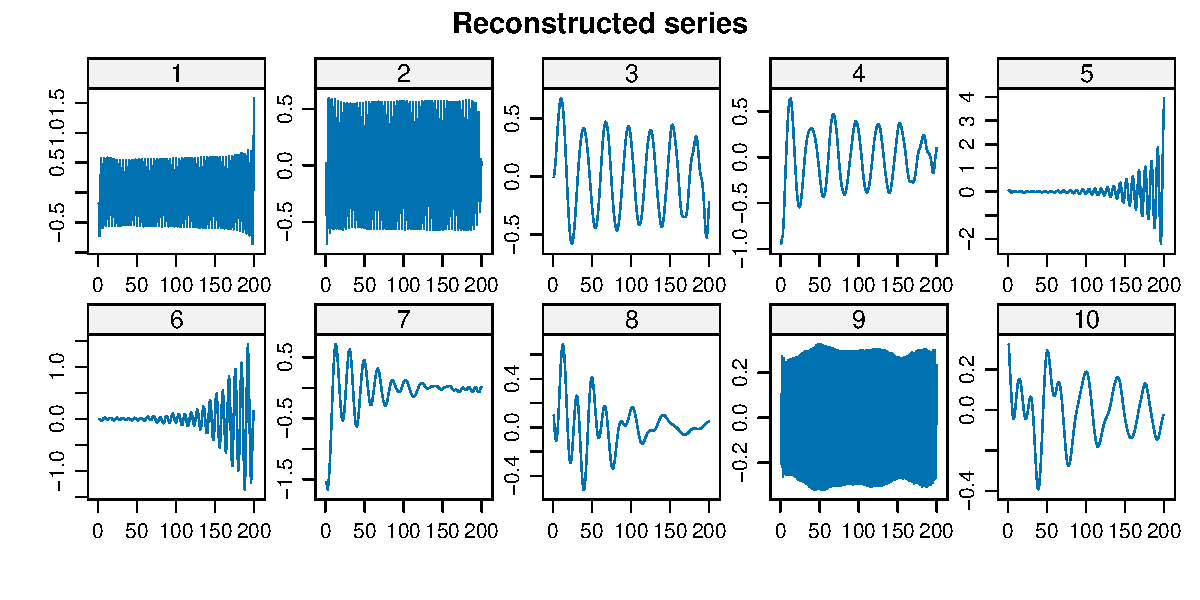
\includegraphics[width=\textwidth]{img/non_dominant_signal_ssa.pdf}
        \caption{Элементарные восстановленные компоненты, $L=96$}
    \end{figure}

    Компоненты, относящиеся к сигналу~--- 1, 2, 5, 6 и 9, однако SSA-Aid обнаружит только первые две компоненты.

\end{frame}

\begin{frame}{Подход к решению проблемы}

    \textcolor{red}{Проблема}: сигнальные компоненты могут оказаться среди шумовых по величине вклада, оставаясь при этом несмешанными с ними.\medskip


    \textcolor{blue}{Идея}: после SSA-Aid использовать другой метод, умеющий определять сигнальные компоненты, не доминирующие над шумом.\medskip

    \textcolor{blue}{Как это сделать}: использовать статистический критерий, который дает информацию о значимых частотах.\medskip

    \textcolor{blue}{Решение}: Monte Carlo SSA (MC-SSA)~[Allen and Smith, 1996] с поправкой на множественные сравнения~[Golyandina, 2023].\medskip

    Также в работе~[Потешкин, 2024] показано, что MC-SSA обладает наибольшей мощностью по сравнению с другими критериями проверки гипотезы об отсутствии сигнала (Q-тест Бокса-Пирса и тест с использованием вейвлетов).

\end{frame}

\begin{frame}{MC-SSA: пример}
    Модель: $\tX=\tS+\bm\xi$, где $\bm\xi$~--- AR(1) с $\phi=0.7$ и $\sigma^2=1$, $N=200$,
    \[
    s_n=0.075e^{0.02n}\cos(2\pi n / 8) + 1.2\cos(2\pi n / 4) + 0.25\cdot (-1)^n.
    \]

    Статистики критерия: $\widehat p_k=\|\bfX^\rmT W_k\|^2$, $W_k=\{\cos(2\pi k n / (2L))\}_{n=1}^L$, $k=1,\ldots,L$. Результат MC-SSA для $L=48$:

    \begin{center}
        
\includegraphics[width=0.7\textwidth]{img/mcssa_real.pdf}
    \end{center}

\end{frame}


\begin{frame}{Метод SSA-AidMC}

    \begin{figure}
        \centering
        
\includegraphics[width=0.82\textwidth]{img/ssa_aidmc_flowchart.pdf}
        \caption{Блок-схема метода SSA-AidMC}
    \end{figure}
    
\end{frame}

\begin{frame}{Метод SSA-AidMC: численное сравнение с методами декомпозиции и прогнозировнаия}

    \footnotesize
    Модель:
    \begin{itemize}
        \item Длина ряда $N=200$.
        \item Тренд $t_n=0.05n$;
        \item Периодика
        \[
        p_n=0.075e^{0.02n}\cos(2\pi n / 8) + 1.5e^{-0.01n}\cos(2\pi n / 4) + 0.8e^{-0.01n}\cdot(-1)^n;
        \]
        \item $\bm\xi$~--- красный шум с параметрами $\phi=0.7$, $\sigma=1$.
    \end{itemize}
   
    \begin{center}
        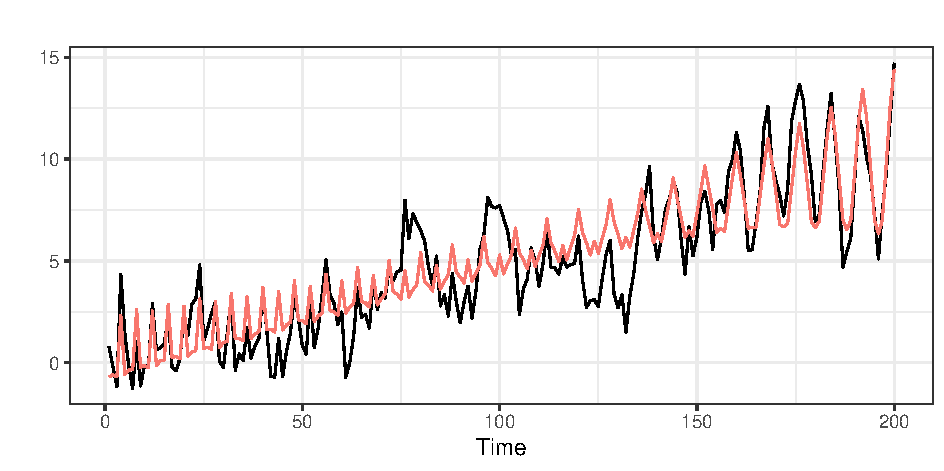
\includegraphics[width=0.8\textwidth]{img/ts_ex.pdf}
    \end{center}

\end{frame}

\begin{frame}{Метод SSA-AidMC: численное сравнение с методами декомпозиции и прогнозировнаия}

    \begin{figure}
        \centering
        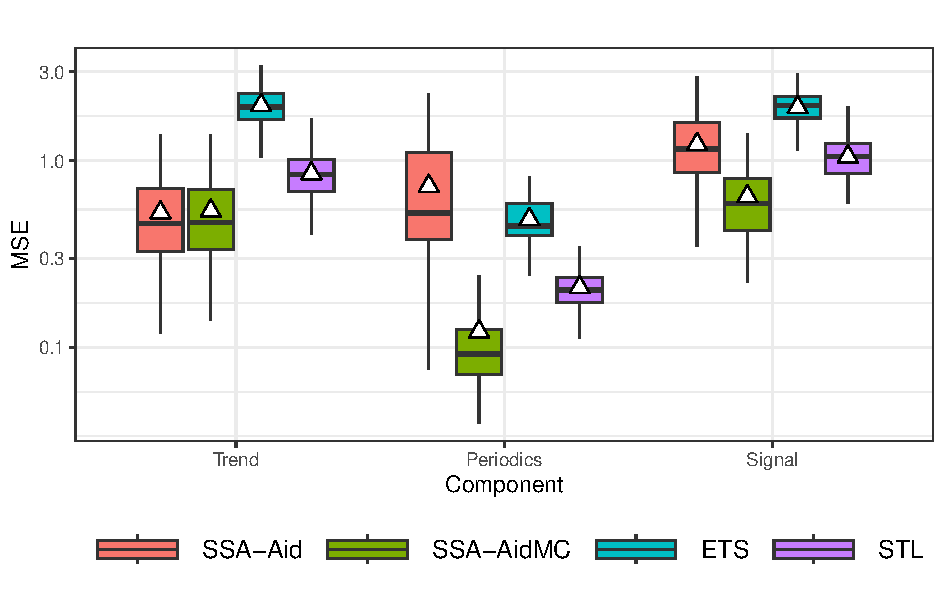
\includegraphics[width=0.82\textwidth]{img/mse_decomposition.pdf}
        \caption{MSE декомпозиции ряда}
    \end{figure}

\end{frame}

\begin{frame}{Метод SSA-AidMC: численное сравнение с методами декомпозиции и прогнозировнаия}

    \begin{figure}
        \centering
        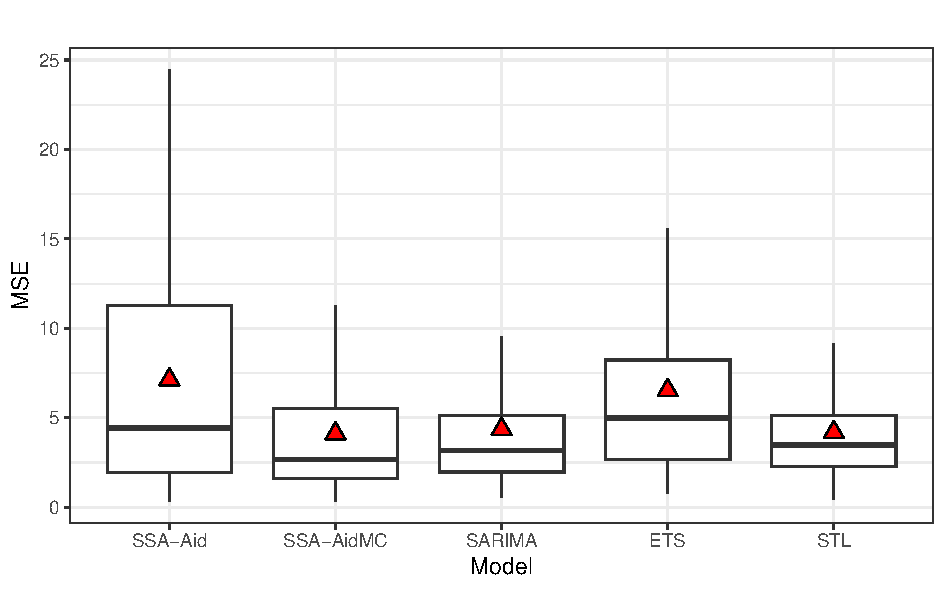
\includegraphics[width=0.82\textwidth]{img/mse_fc.pdf}
        \caption{MSE прогноза на один период ($h=8$)}
    \end{figure}

\end{frame}

\begin{frame}[plain, noframenumbering]{Пример результата прогноза}

    \begin{figure}
        \centering
        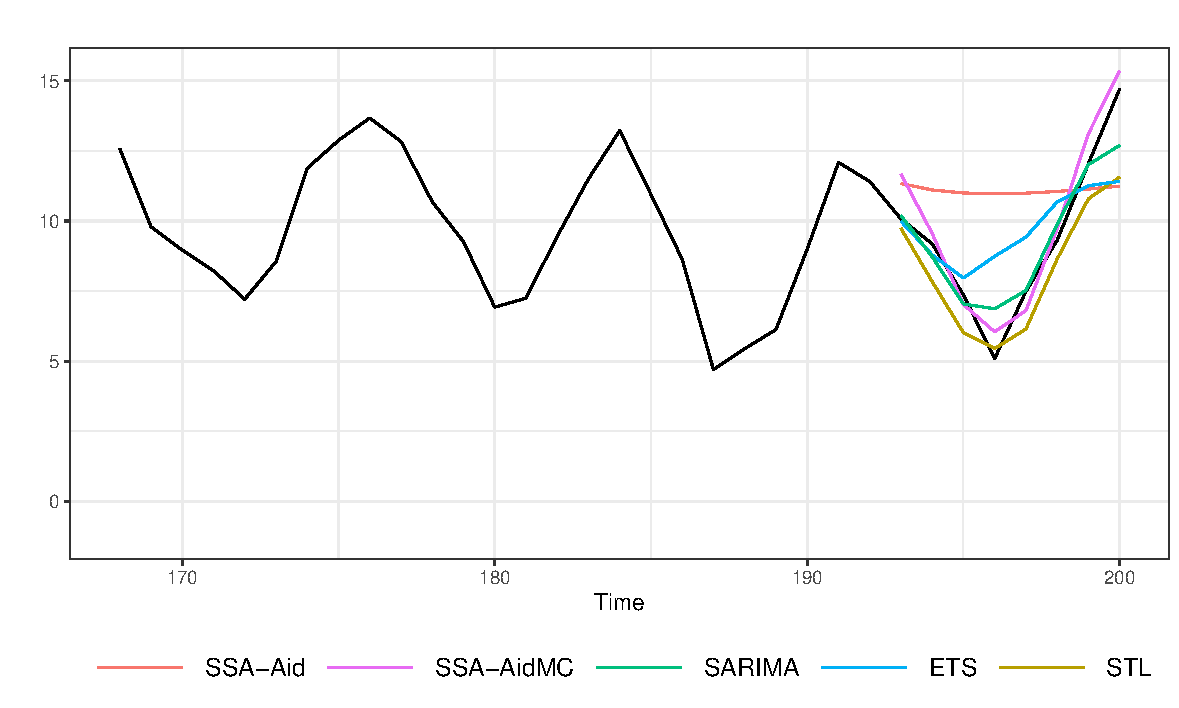
\includegraphics[width=\textwidth]{img/ts_ex_fc.pdf}
        \caption{Прогноз на один период}
    \end{figure}

\end{frame}

\begin{frame}[plain, noframenumbering]{Список литературы}

    \begin{thebibliography}{9}
        \bibitem{Broomhead_King_1986}
        Broomhead D. S., King G. P. Extracting qualitative dynamics from experimental data // Physica D: Nonlinear Phenomena. — 1986. — Vol. 20, no. 2–3. — P. 217–236.

        \bibitem{Golyandina_Nekrutkin_Zhigljavsky_2001}
        Golyandina N., Nekrutkin V., Zhigljavsky A. Analysis of Time Series Structure. — Chapman and Hall/CRC, 2001.

        \bibitem{Shlemov_2017}
        Шлемов А. Метод разделения сигналов с использованием собственных подпространств сдвиговых матриц // Материалы всероссийской научной конференции по проблемам информатики СПИСОК-2017. — 2017. — С. 486 – 496.

        \bibitem{Golyandina_Dudnik_Shlemov_2023}
        Golyandina N., Dudnik P., Shlemov A. Intelligent Identification of Trend Components in Singular Spectrum Analysis // Algorithms. — 2023. — Vol. 16, no. 7.

        \bibitem{Zhornikova_2018}
        Жорникова П. Идентификация компонент в анализе сингулярного спектра : квалификационная работа магистра ; СПбГУ. — 2018.

        \bibitem{Dudnik_2025}
        Дудник П. Идентификация компонент временных рядов в методе SSA : квалификационная работа магистра ; СПбГУ. — 2025.

    \end{thebibliography}

\end{frame}

\begin{frame}[plain, noframenumbering]{Список литературы}
    
    \begin{thebibliography}{9}
        \bibitem{Allen_Smith_1996}
        Allen M. R., Smith L. A. Monte Carlo SSA: Detecting irregular oscillations in the Presence of Colored Noise // Journal of Climate. — 1996. — Vol. 9 no. 12. — P. 3373–3404.

        \bibitem{Golyandina_2023}
        Golyandina N. Detection of signals by Monte Carlo singular spectrum analysis: multiple testing // Statistics and Its Interface. — 2023. — Vol. 16, no. 1. — P. 147–157.

        \bibitem{Poteshkin_2024}
        Потешкин Е. Метод Монте-Карло SSA для одномерных и многомерных временных рядов : квалификационная работа бакалавра ; СПбГУ. — 2024.

        \bibitem{Box_Pierce_1970}
        Box G. E. P., Pierce D. A. Distribution of Residual Autocorrelations in Autoregressive-Integrated Moving Average Time Series Models // Journal of the American Statistical Association. — 1970. — Vol. 65, no. 332. — P. 1509–1526.

        \bibitem{Nason_Savchev_2014}
        Nason G. P., Savchev D. White noise testing using wavelets // Stat. — 2014. — Vol. 3, no. 1. — P. 351–362.
    \end{thebibliography} 

\end{frame}

\end{document}